\section{\textbf{Transmission Design}}
\label{sec:transmissionDesign}

The actuator design philosophy is to make high power actuators with the capability of interacting with the environment. Namely, the actuator should not be stiff as the heavily geared motors, which are widely used in industrial robots. Instead, it should be back-drivable meaning that the torque applied at the output shaft should be felt at the input shaft. The benefits are threefold, firstly, back-drivability prevents geatboxes from being damaged by external forces; second, it allows for proprioceptive sensing\cite{Seok2012}; thirdly, allows for fast dynamics in legged locomotion.

After the motor selection and gear ratio is determined from previous sections, focus was put on how to design the transmission system so that it can achieve the desired gear ratio while satisfying dimensional constraints.

\subsection{\textbf{Transmission Design Comparison}}
\label{sec:transmissionComparison}

\textbf{Harmonic drive} is composed of the wave generator, flexspline and circular spline. It could provide high gear ratio typically between 30:1 to 200:1 with zero backlash. Harmonic drive is employed by the quadrupedal robot starlETH\cite{Hutter2013} and the bipedal robot ATRIAS\cite{Hubicki2016}. However, harmonic drive is not back-drivable, which contradicts with our design paradigm.

\textbf{Cycloidal gearbox} has very low backlash and high torsional stiffness. It can operate quietly and withstand shock load. Bipedal robot Cassie uses cycloidal gearbox as the transmission. The drawback of cycloidal gearbox is that it requires customizing high precision parts.

\textbf{Single stage planetary gearbox} has high efficiency and the load could be distributed between planet gears, and standard gears are widely available at low cost. Nevertheless, no gear combination could provide the desired gear ratio for the given dimensional limitation with pitch of 0.4.

\textbf{Compound planetary gearboxes} have the benefits of single stage planetary gearboxes while providing more compact design for there are two stages for the planet gear. There are a range of gear teeth selection for the given dimensional limits. It is adopted as the transmission system design considering the dimensional limit and gear ratio requirement of the motor design.

\subsection{\textbf{Compound Planetary Gearbox Design}}
\label{sec:compoundGearBox}

\begin{figure}
	\centering
	\resizebox{1.0\linewidth}{!}{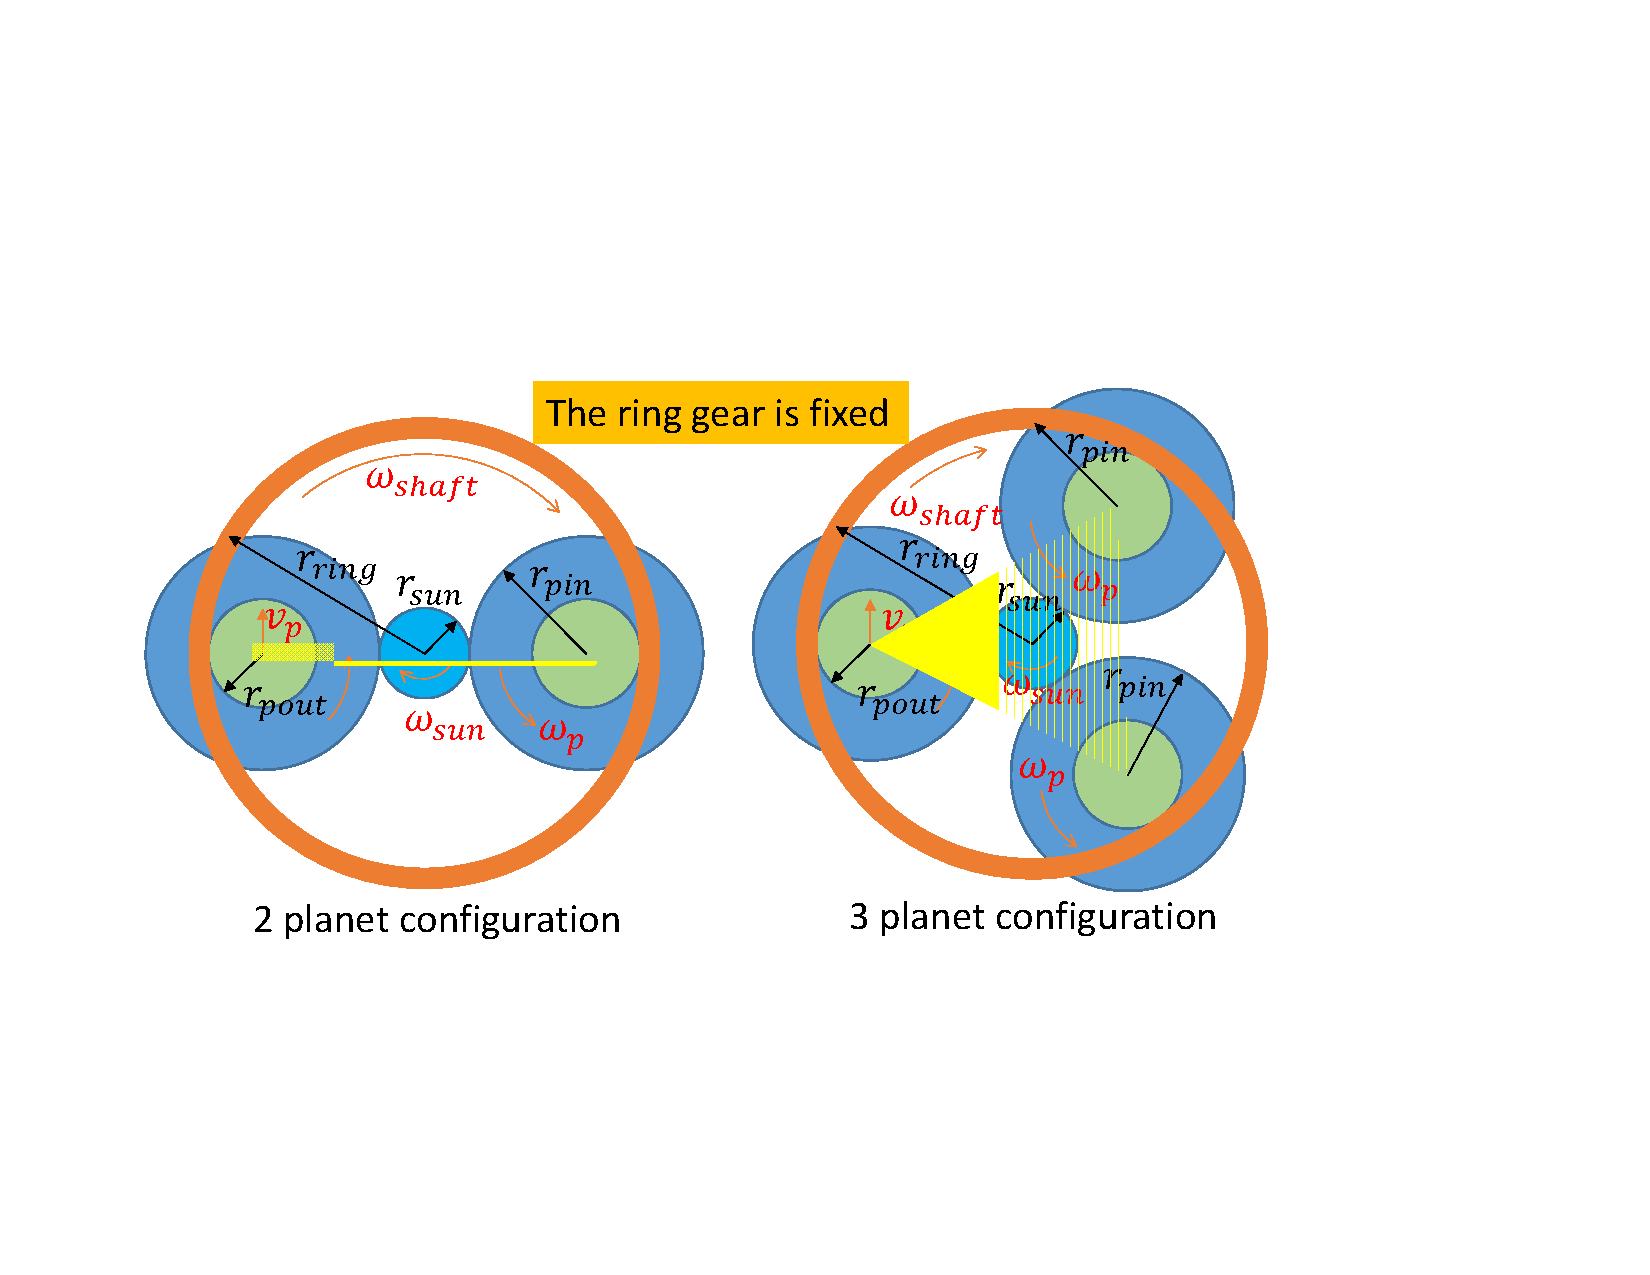
\includegraphics{planetaryGearbox.pdf}}
	\caption{Schematics of Compound Planetary Gearbox Configurations. (left) 2 planet configuration, (right) 3 planet configuration}
	\label{fig:planetaryGearbox}
\end{figure}

The objective of compound planetary gearbox design is to achieve desired gear ratio within dimensional constraints imposed by motor selection. In order to derive the gear ratio for given gear teeth number, a schematics of the two-stage compound planetary gearbox is used as shown in Figure \ref{fig:planetaryGearbox}. For given gear teeth numbers, both configurations in Figure \ref{fig:planetaryGearbox} are equivalent. Some assumptions for this analysis is posed here: 

\begin{enumerate}
	\item The sun gear located at the center is the input.
	\item The output shaft shown as yellow transparent shape is the output.
	\item The output shaft is connected to the axes of all the planet gears.
	\item The sun gear is meshed with input planet gears.
	\item The ring gear is meshed with output planet gears.
	\item The ring gear is fixed.
\end{enumerate}

Velocity equivalence is used to calculate the gear ratio.
\begin{eqnarray}
\omega_{sun} r_{sun} =& v_p + \omega_p r_{pin}\\
v_p =& \omega_{p} r_{pout}\\
\omega_p =& \frac{\omega_{sun}r_{sun}}{r_{pout}+r_{pin}}\\
\omega_{shaft} =& \frac{\omega_{p}r_{pout}}{r_{sun}+r_{pin}}
\end{eqnarray}
where $\omega_{shaft}$ is the angular velocity of the output shaft and the rest of the variable definitions could be found in Table \ref{tab:varDefGearbox}.

Therefore, the gear ratio of a compound planetary gearbox could be formulated as:
\begin{equation}
GR = \frac{\omega_{sun}}{\omega_{shaft}} = \frac{(r_{pout}+r_{pin})(r_{sun}+r_{pin})}{r_{sun}r_{pout}} = \frac{(N_{pout}+N_{pin})(N_{sun}+N_{pin})}{N_{sun}N_{pout}}
\end{equation}

\begin{table}[bp]
	\centering
	\caption{Variable Definition for Gear Ratio Calculation}
	\begin{tabular}{lcccc}\hline\hline
		& Sun gear		& Input planet	& Output planet	& Ring gear \\ \hline
		Pitch diameter	& $r_{sun}$	   	& $r_{pin}$		& $r_{pout}$	& $r_{ring}$\\
		Angular velocity& $\omega_{sun}$& $\omega_{p}$	& $\omega_{p}$	& N/A		\\
		Linear velocity	& N/A			& $v_p$			& $v_p$			& N/A		\\
		Teeth number	& $N_{sun}$		& $N_{pout}$	& $N_{pout}$	& $N_{ring}$\\ \hline
	\end{tabular}
	\label{tab:varDefGearbox}
\end{table}

The planetary gearbox shown in Figure \ref{fig:gearbox} utilizes two-stage compound planet gears to provide desired gear ratio while satisfying the dimensional constraints imposed by motor selection. 

A large number of teeth combinations were enumerated and the optimal gear teeth choice emerged (GR = 23.36; sun gear: 12; planet gear: 16/53; ring gear: 81). The constraints for choosing teeth numbers are listed as follows:

\begin{enumerate}
	\item The teeth number of sun gear ($N_{sun}$) and ring gear ($N_{ring}$) could both be divided by the number of planet gears.
	\item The pitch circles of sun gear and planet gears, as well as that of planet gears and the ring gear should be externally tangent, 
	
	i.e. $r_{ring}=r_{sun}+r_{pin}+r_{pout}$ or $N_{ring}=N_{sun}+N_{pin}+N_{pout}$.
	\item The gear ratio $GR$ should be within the range of 22 - 25.
	\item The radius of the gearbox should be less than 25 mm, 
	
	i.e. $Max[r_{ring},r_{sun}+2r_{pin}]<12.5 mm$
	\item The teeth number for sun gear $N_{sun}$ should be no less than 6. Other wise the meshing would be problematic because the profile of gear teeth would be distorted too much.
\end{enumerate}

 Ideally, the phase difference between two stages should be the same for all compound planet gears. However, in compound gear manufacturing, the phase differnce could not be well maintained. To solve this problem, the planet gear teeth combination was chosen to be 16/53, which only share the common factor of 1. This choice provides tunable backlash with $2.1^{\circ}$ increment in the gearbox assembly. This is very similar to the working principle of a mechanical caliper, which uses two scales (main scale and vernier scale) with small difference to achieve high precision.

\section{\textbf{Mechanical Design of The Leg}}
\label{sec:LegDesign}

With actuator from $\color{red}section$ and linkage design from $\color{red}section$, this section presents a detailed mechanical design layout of the leg. The leg module is composed of three motor modules(HIP/KNEE/ABAD), each has a motor coil and a planetary gearbox with moderate gear ratio to achieve the Quasi-Direct-Drive\cite{20162016} strategy. To accommodate size limitation imposed by actuator choice, the two-stage compound planetary gearbox is used as the transmission. The leg is design to optimize for large workspace, with the novel HIP-KNEE connection design, the knee joint could rotate $360^{\circ}$, the curved upper link and hollow thigh link design also enables large knee joint workspace.
  
\begin{figure}
	\centering
	\resizebox{1\linewidth}{!}{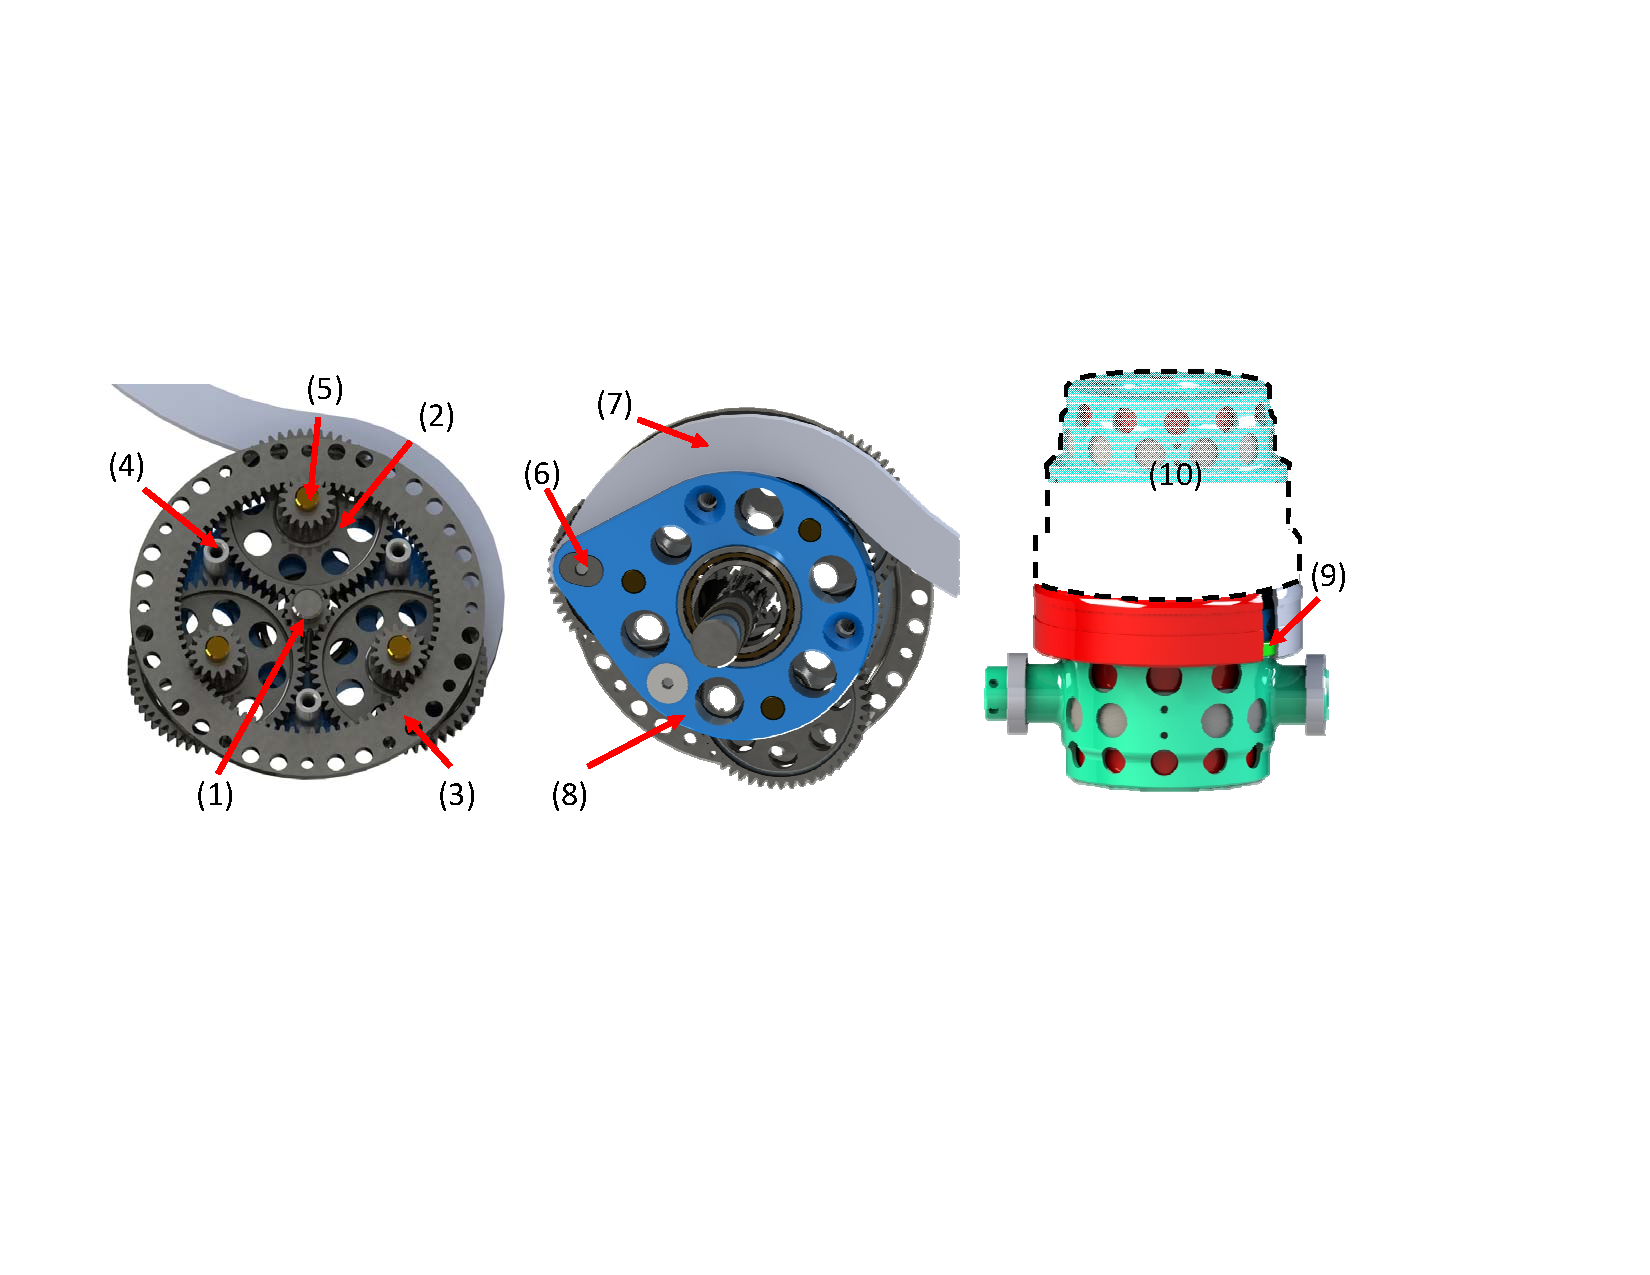
\includegraphics{gearbox.pdf}}
	\caption{Planetary gearbox design with three compound planet gears (left); curved upper-link design (middle); hip and knee motor module (right); (1) sun gear, (2) compound planet gear, (3) ring gear, (4) stand-off, (5) brass dowel pin, (6) output pin, (7) upper link, (8) KNEE carrier, (9) KMF PBXS020 bearing, (10) the KNEE motor module}
	\label{fig:gearbox}
\end{figure}



\subsection{\textbf{HIP-KNEE Connection Design}}
\label{sec:Design4ROM}

\begin{figure}
	\centering
	\resizebox{1.0\linewidth}{!}{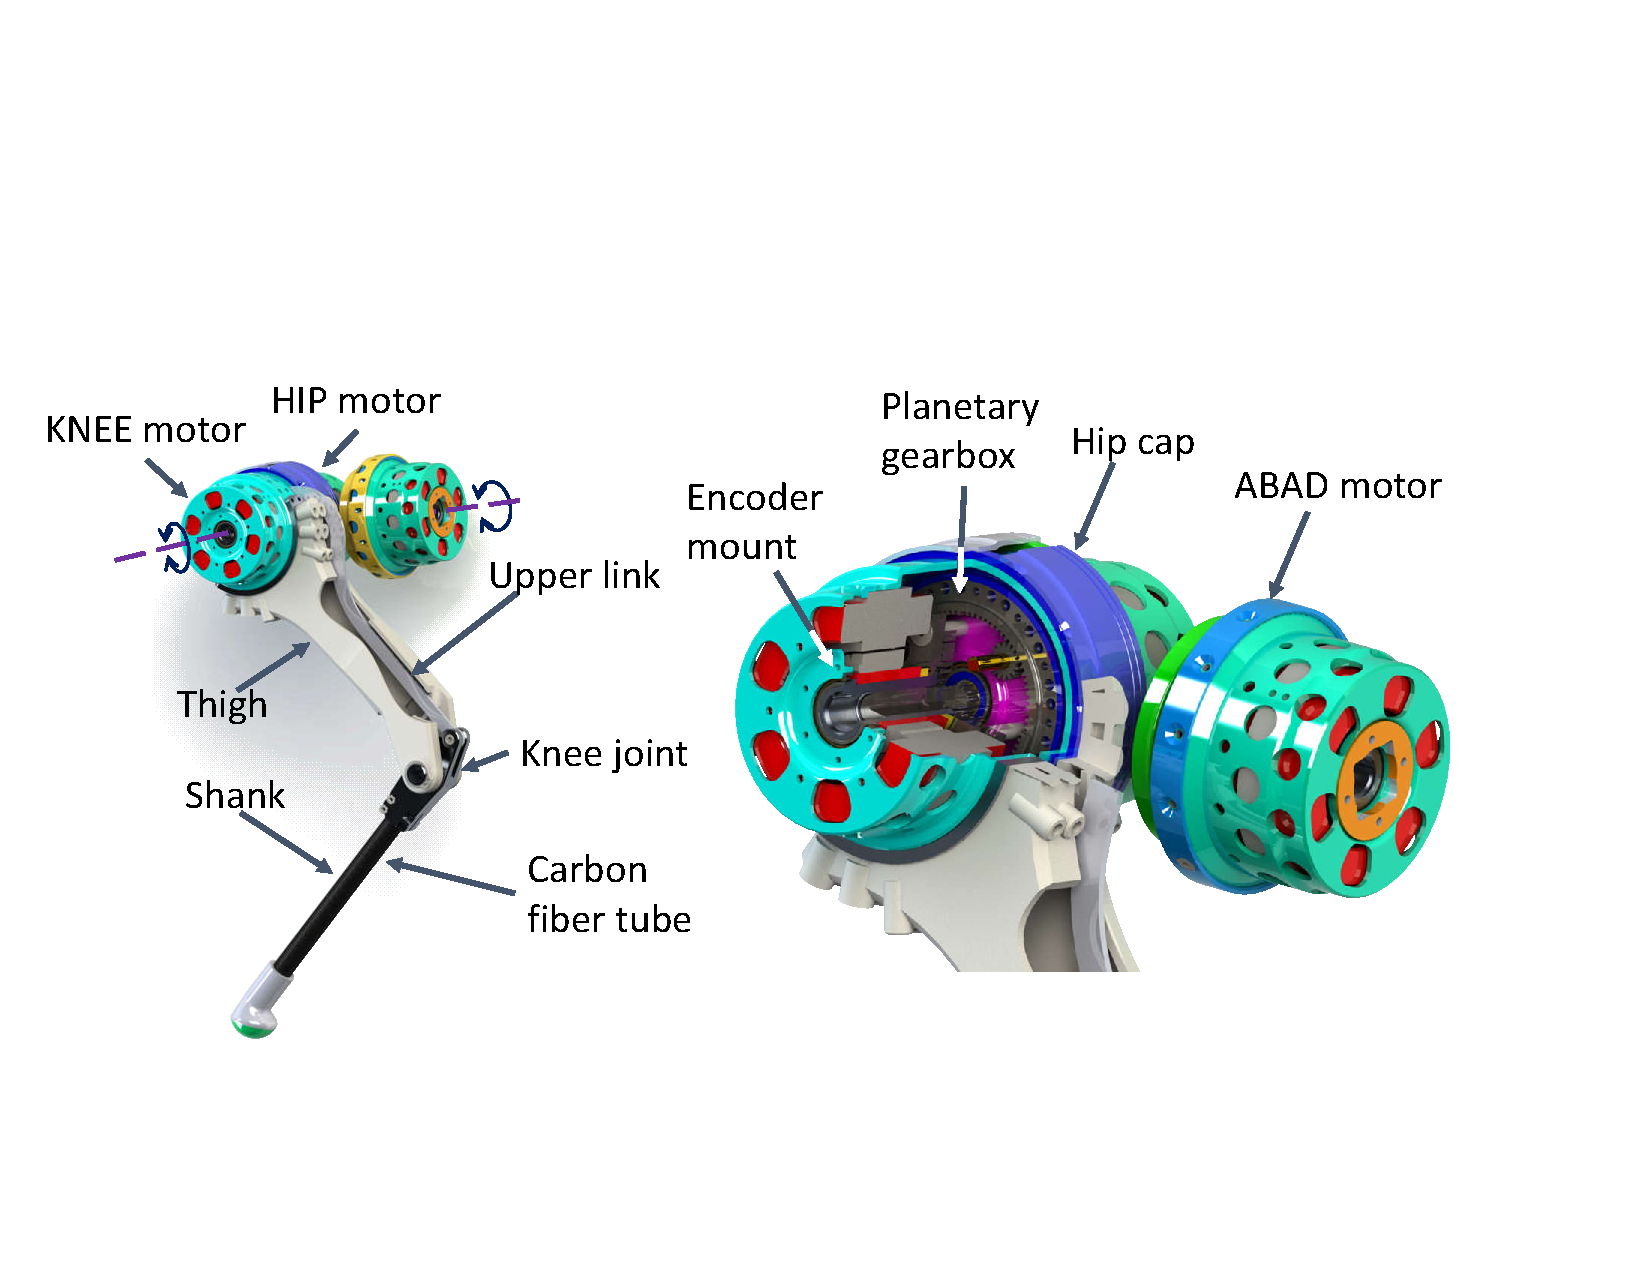
\includegraphics{SWrendering.pdf}}
	\caption{CAD Model of the Leg Module Design; (left) A side-view of the leg module with cut-out on thigh link showing the four-bar linkage design; (right) A cut-out view showing the internal structure of a motor module}
	\label{fig:LegDesign}
\end{figure}
\begin{figure}
	\centering
	\resizebox{1.0\linewidth}{!}{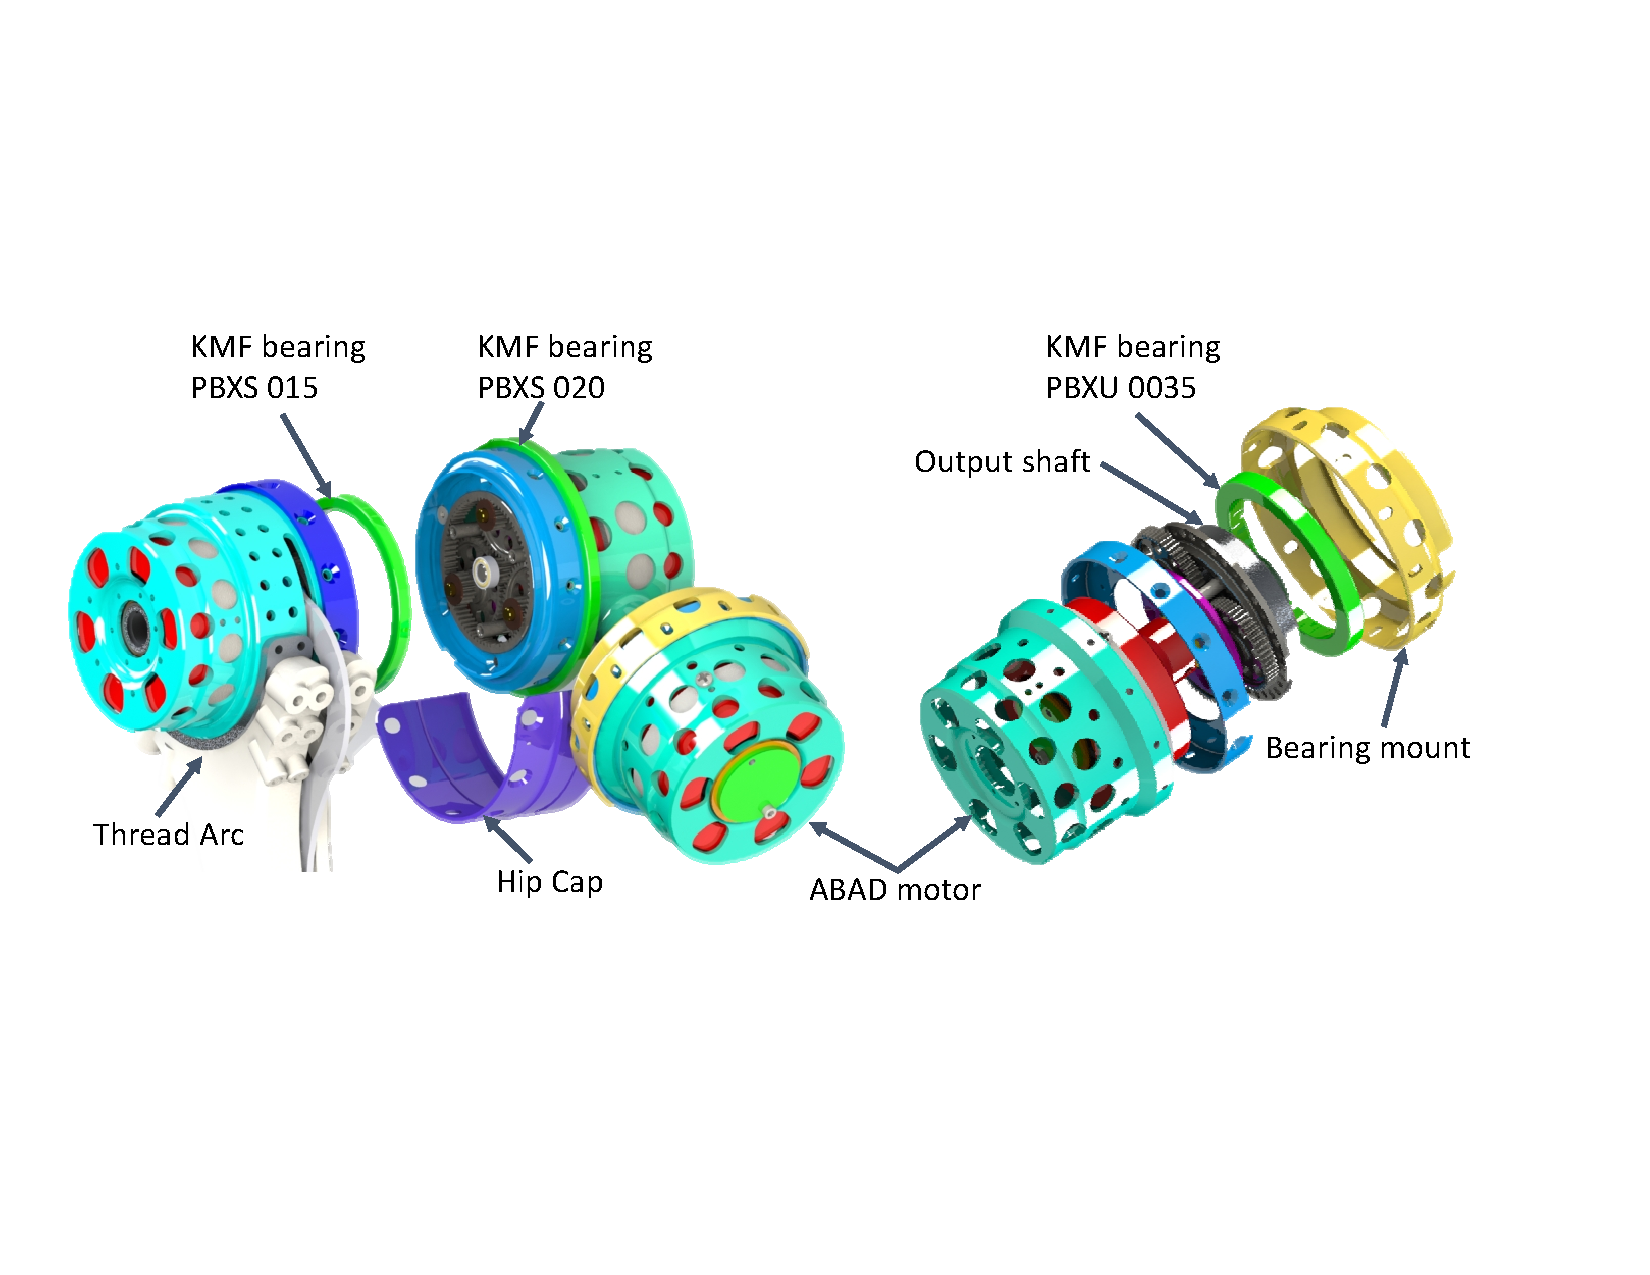
\includegraphics{KMFbearings.pdf}}
	\caption{(left) Connection Design Between HIP and KNEE Motors for Large Hip Range of Motion (ROM); (right) Exploded View of ABAD motor}
	\label{fig:KMFbearings}
\end{figure}

Each leg module is composed of three brush-less DC (BLDC) motor modules. HIP, KNEE, ABAD stand for hip joint, knee joint and abduction/adduction joints respectively. The HIP and KNEE motors are placed face-to-face and coaxially as shown in Figure \ref{fig:LegDesign}. Double supported by two thin-section bearings (KMF: PBXS020/ PBXS015), the KNEE motor could rotate $360^{\circ}$ with respect to the HIP motor. One bearing (KMF: PBXS015) is located between HIP and KNEE motors and the other one (PBXS020) is located outside of the HIP motor shell and enclosed by two hip caps. An explosive view could be found in Figure \ref{fig:KMFbearings}. The HIP motor shell's outer surface is used as one of bearing PBXS020's mating surface, and the inner surface of the Hip cap is used as the other mating surface. The hip cap is fixed to the KNEE motor and grips on the HIP motor via PBXS020 bearing, allowing the KNEE motor to rotate freely related to the HIP motor.

The ABAD motor's rotational axis is placed perpendicular to the HIP/KNEE motors' axis. The internal structure of the ABAD motor is shown in Figure \ref{fig:KMFbearings}. The torque produced by electrical coil is magnified by the planetary gearbox and transfered to the output shaft, whose motion is constrained by the bearing mount via another thin-section bearing(KMF PBXU0035). The output shaft of ABAD motor is directly connected to the HIP/KNEE module. With transmission eliminated, the workspace of the ABAD joint is not limited by the leg itself. 

\subsection{\textbf{Linkage Transmission Design}}
\label{sec:legDesign}

The linkage transmission design is shown in Figure \ref{fig:LegDesign}. The torque of the KNEE motor is transmitted to the knee joint through a four-bar linkage mechanism. Hence the KNEE motor could be put nearer to the main body and the rotary inertia could be reduced. The 3D printed hollow thigh design allows the curved upper link to travel inside without interference, while providing protection to the upper link. Consequently, the robot-human interface would be safer. In addition, the curved upper link design allows larger knee joint workspace compared with straight link design As shown in Figure \ref{fig:gearbox}, the curved link avoids the standoff (4) in the figure and gains $27^{\circ}$ more rotation angle compared with straight four-bar linkage design.

The thigh link was connected to the KNEE motor surface through four screws initially. During preliminary jumping tests it turned out that the large ground impact impulse at touch down would rip off the thread on the KNEE motor shell. To solve this problem, an additional part called thread arc was made to provide more threaded holes on the knee motor. Figure \ref{fig:KMFbearings} shows that the thread arc is attached to the KNEE motor surface and the new thigh link is fixed to the thread arc with 18 screws to evenly distribute the load.

\subsection{\textbf{Electronic System Integration}}
\label{sec:Electronics}

The electronic system of the robot leg consists of the following components: two Elmo Gold Twitter amplifiers were used for motor commutation, two RLS-RMB20 magnetic encoders were used to measure motor angle, ATI Mini40 F/T sensor was used to measure the ground reaction force created by the leg. The control loop runs at 4kHz on an Intel i5 desktop in Simulink Real-Time. 


